%%---------------------------------------------Binary Mixtures--------------------------------------------------%%
%%--------------------------------------------------------------------------------------------------------------%%

\section{Binary Mixtures}

The bi-level optimization method for parameter estimation was successfully applied using the Python programming language. Multi-parameter, constrained optimizers included in the SciPy.Optimize package were used. This method was however found to be very sensitive to initial values and convergence was unreliable. The software would often terminate after a large number of iterations, or function evaluations, without converging to a feasible solution. This is probably due to the complexity of the unknown overall or underlying mathematical function.\\

In order to overcome this, calculation of binary interaction parameters at various temperatures required manual tweaking of initial parameter guesses for each system, for each model. This is tedious, inconvenient and very problematic for cases where the range or order of magnitude of the interaction parameters is unknown. These optimizations may take hours to perform, with no guarantee of convergence to a stable equilibrium solution.\\

Another problem which was encountered with the use of the bi-level optimization approach is that of parameter scaling. When the range of possible binary interaction parameters is large, and the parameters being evaluated differ greatly in magnitude, scaling issues may prevent the optimization technique from converging.\\

Consistent, repeatable results could not be obtained for all binary mixtures using the bi-level optimization approach, due to the difficulties experienced with the implementation thereof. The parameters and phase diagrams for each of the models and each of the binary mixtures in table \ref{BinarySystemsandReferences} where instead calculated using the pseudo-analytical approach discussed in section \ref{BinaryPAMethodSection}. It was found that this method converged reliably.\\

The pseudo analytical approach does apply a random multi-start approach. This is done in order to ensure convergence to physically significant solutions. However, each solution is readily tested for compliance to certain requirements. This process is automated and therefore requires no manual tweaking. For example, in the case of calculated phase equilibrium compositions, $\sum_{i}^{n} x_{i} = 1$ must apply. Also, the predicted tie-line must have a negative value at $x=0$ and $x=1$. Nevertheless, the pseudo analytical method converged very rapidly, and reliably, in spite of the use of a multi-start approach.\\

For the DWPM the values of $s_{i}$ in equation \ref{DWPMWilsonLike} are chosen as $\nicefrac{1}{2}$. Therefore, the form of the DWPM model used in this investigation reduces to the 3 parameter Wilson model. For the binary systems investigated here, this provides sufficient flexibility to accurately model the experimental phase behaviour. The software is however programmed to accommodate any values for each $s_{i}$, and the pseudo analytical approach converges equally easily and rapidly for any sensible combination of these parameters.\\

The current pseudo analytical approach utilises a system of four equations to calculate four unknowns. It is based on the experimentally measured information of one tie-line. In the case of most binary systems, which exhibit no more than one miscibility gap, it is therefore sufficient to arbitrarily specify the $s_{i}$ parameters and vary the binary interaction parameters to match the experimental data. However, if more complex phase behaviour needs to be correlated, the flexibility of the DWPM model becomes useful. Using a similar equation solving approach as before, a set of equations can be formulated to enforce multiple miscibility gaps.\\

For example, consider a hypothetical binary liquid mixture for which two liquid phase splits, at a given temperature, have been observed experimentally. Using the four experimentally measured phase compositions, a system of eight equations and eight unknowns can be formulated:\

\begin{eqnarray}
g\left(x_{\alpha}\right) &=& f\left(x_{\alpha}\right) \label{BianryMultipleSplitEqs1}\\
\frac{\mathrm{d}g\left(x_{\alpha}\right)}{\mathrm{d}x_{1}} &=& \frac{\mathrm{d}f\left(x_{\alpha}\right)}{\mathrm{d}x_{1}}\\
g\left(x_{\beta}\right) &=& f\left(x_{\beta}\right)\\
\frac{\mathrm{d}g\left(x_{\beta}\right)}{\mathrm{d}x_{1}} &=& \frac{\mathrm{d}f\left(x_{\beta}\right)}{\mathrm{d}x_{1}}\\
g\left(x_{\gamma}\right) &=& f\left(x_{\gamma}\right)\\
\frac{\mathrm{d}g\left(x_{\gamma}\right)}{\mathrm{d}x_{1}} &=& \frac{\mathrm{d}f\left(x_{\gamma}\right)}{\mathrm{d}x_{1}}\\
g\left(x_{\phi}\right) &=& f\left(x_{\phi}\right)\\
\frac{\mathrm{d}g\left(x_{\phi}\right)}{\mathrm{d}x_{1}} &=& \frac{\mathrm{d}f\left(x_{\phi}\right)}{\mathrm{d}x_{1}}\label{BianryMultipleSplitEqs2} 
\end{eqnarray}\

Where $x_{\alpha}$ and $x_{\beta}$ are the experimental tie-line compositions of the first phase split, and $x_{\gamma}$ and $x_{\phi}$ that of the second. As before, $g\left(x_{1}\right) = \dfrac{G\left(x_{1}\right)}{RT}$. $f_{1}\left(x_{1}\right)$ is the common tangent line to the Gibbs energy curve at $x_{\alpha}$ and $x_{\beta}$, and $f_{2}\left(x_{1}\right)$ the common tangent at $x_{\gamma}$ and $x_{\phi}$:\

\begin{eqnarray}
f_{1}\left(x_{1}\right) = m_{1}x_{1} + c_{1} \\
f_{2}\left(x_{1}\right) = m_{2}x_{1}+ c_{2} 
\end{eqnarray}\

By solving the system in equations \ref{BianryMultipleSplitEqs1} to \ref{BianryMultipleSplitEqs2} the two binary interaction parameters, $\Lambda_{ij}$ and $\Lambda_{ji}$, as well as $s_{1}$, $s_{2}$, $m_{1}$, $m_{2}$, $c_{1}$ and $c_{2}$ can be calculated. Thereby enforcing the thermodynamic behaviour required to represent the physical system. While this has not currently been applied, it could be the subject of a future investigation.\\

In the current investigation, $\alpha$ is chosen as 0.2 for the NRTL model, where $\alpha= \alpha_{ij}=\alpha_{ji}$. The pure component constants, $r_{i}$ and $q_{i}$, for the UNIQUAC model are supplied in the Dechema data collection~\cite{Dechema}. The calculated binary interaction parameters for each of the binary mixtures, using the NRTL, UNIQUAC and DWPM models are now presented.\\


%%2-Hexanol-Water--------------------------------------------------------------------------------------------------%

The calculated binary interaction parameters for the mixture 2-Hexanol and Water, for each of the models, at the experimental temperatures is displayed in table \ref{2HexanolWaterTable}. The phase diagram predicted by the DWPM, NRTL and UNIQIAC models, using 10 sets of linearly interpolated parameters, and the original experimentally measured phase compositions are displayed in figure \ref{hexanol-waterFigure}.\\

\begin{landscape}
\vspace*{\fill}
\begin{table}[h]
\caption{Calculated binary interaction parameters for 2-Hexanol and Water} 
\centering
\begin{tabular}{lcccccc}
\toprule
\textbf{Temperature}/$\mathrm{K}$&\multicolumn{2}{c}{\textbf{NRTL}}&\multicolumn{2}{c}{\textbf{UNIQUAC}}&\multicolumn{2}{c}{\textbf{DWPM}}\\
\cmidrule(r){2-7}
&$g_{ij}$&$g_{ji}$&$u_{ij}$&$u_{ji}$&$\Lambda_{ij}$&$\Lambda_{ji}$\\
\midrule
\textbf{ 293.00 } & \num{-1.011d2} & \num{1.788d3} & \num{1.780d2} & \num{1.659d2} & \num{2.423d-3} & \num{1.159}\\
\textbf{ 298.00 } & \num{-1.086d2} & \num{1.850d3} & \num{1.684d2} & \num{1.820d2} & \num{2.169d-3} & \num{1.184}\\
\textbf{ 303.00 } & \num{-1.164d2} & \num{1.906d3} & \num{1.607d2} & \num{1.953d2} & \num{2.000d-3} & \num{1.209}\\
\bottomrule
\end{tabular}\\
\label{2HexanolWaterTable}
\end{table}
\vspace*{\fill}
\end{landscape}

\begin{figure}[hp]
\centering
\includegraphics[width = 0.85\textwidth]{Results_Parts/BinaryParams/2-hexanol-water/PhaseDiagram.eps}
\caption{Calculated phase diagram for 2-Hexanol and Water} \label{hexanol-waterFigure}
\end{figure}\

\clearpage 

For each of the binary mixtures modelled, the $\Delta G_{mix}$ curves, and resulting phase splits, predicted by the NRTL, UNIQUAC and DWPM models are included in the Appendix in section \ref{AppendixGibbsPlotsBinaries}. For each of these plots the change of Gibbs energy on mixing versus composition is determined using the set of calculated interaction parameters, at the relevant temperatures. \\


%%13-Dimethyl Benzene and Water-----------------------------------------------------------------------------------%%

The calculated parameters for 13-Dimethyl Benzene and Water for each model, at the experimental temperatures is displayed in table \ref{13DimethylBenzeneWaterTable}. As before, the phase diagram predicted by the DWPM, NRTL and UNIQIAC models, using 10 sets of linearly interpolated parameters, and the original experimentally measured phase compositions are displayed in figure \ref{13DimethylBenzeneWaterFigure}.\\

\begin{landscape}
\vspace*{\fill}
\begin{table}[h]
\caption{Calculated binary interaction parameters for 13-Dimethyl Benzene and Water}
\centering
\begin{tabular}{lcccccc}
\toprule
\textbf{Temperature}/$\mathrm{K}$&\multicolumn{2}{c}{\textbf{NRTL}}&\multicolumn{2}{c}{\textbf{UNIQUAC}}&\multicolumn{2}{c}{\textbf{DWPM}}\\
\cmidrule(r){2-7}
&$g_{ij}$&$g_{ji}$&$u_{ij}$&$u_{ji}$&$\Lambda_{ij}$&$\Lambda_{ji}$\\
\midrule
\textbf{ 292.85 } & \num{1.386d3} & \num{2.541d3} & \num{1.000d3} & \num{3.371d2} & \num{1.579d-4} & \num{1.352d-2}\\
\textbf{ 312.85 } & \num{1.265d3} & \num{2.626d3} & \num{9.282d2} & \num{3.376d2} & \num{1.987d-4} & \num{2.588d-2}\\
\textbf{ 342.85 } & \num{1.033d3} & \num{2.741d3} & \num{7.842d2} & \num{3.337d2} & \num{2.808d-4} & \num{6.865d-2}\\
\bottomrule
\end{tabular}\\
\label{13DimethylBenzeneWaterTable}
\end{table}
\vspace*{\fill}
\end{landscape}

\begin{figure}[hp]
\centering
\includegraphics[width = 0.85\textwidth]{Results_Parts/BinaryParams/13-dimethylbenzene-water/PhaseDiagram.eps}
\caption{Calculated phase diagram for 13-Dimethyl Benzene and Water} \label{13DimethylBenzeneWaterFigure}
\end{figure}\

\clearpage

%% Aniline and Water----------------------------------------------------------------------------------------------%%

The results for the mixture Aniline and Water for each model, at the experimental temperatures are displayed in table \ref{AnilineWaterTable}. The calculated phase diagrams using the DWPM, NRTL and UNIQIAC models are presented in figure \ref{aniline-waterFigure}. The binary interaction parameters were again linearly interpolated at 9 equally spaced intervals for the construction of the phase diagrams. 

\begin{landscape}
\vspace*{\fill}
\begin{table}[h]
\caption{Calculated binary interaction parameters for Aniline and Water} 
\centering
\begin{tabular}{lcccccc}
\toprule
\textbf{Temperature}/$\mathrm{K}$&\multicolumn{2}{c}{\textbf{NRTL}}&\multicolumn{2}{c}{\textbf{UNIQUAC}}&\multicolumn{2}{c}{\textbf{DWPM}}\\
\cmidrule(r){2-7}
&$g_{ij}$&$g_{ji}$&$u_{ij}$&$u_{ji}$&$\Lambda_{ij}$&$\Lambda_{ji}$\\
\midrule
\textbf{ 281.60 } & \num{1.944d1} & \num{1.384d3} & \num{1.576d2} & \num{1.056d2} & \num{7.805d-3} & \num{7.746d-1}\\
\textbf{ 298.40 } & \num{-4.970d1} & \num{1.510d3} & \num{9.818d1} & \num{1.465d2} & \num{6.999d-3} & \num{9.409d-1}\\
\textbf{ 321.00 } & \num{-4.920d1} & \num{1.582d3} & \num{1.283d2} & \num{1.290d2} & \num{7.994d-3} & \num{9.237d-1}\\
\textbf{ 339.30 } & \num{-9.394d1} & \num{1.655d3} & \num{1.166d2} & \num{1.281d2} & \num{8.663d-3} & \num{1.011}\\
\textbf{ 369.70 } & \num{-2.231d2} & \num{1.800d3} & \num{5.003d1} & \num{1.518d2} & \num{9.514d-3} & \num{1.273}\\
\bottomrule
\end{tabular}\\
\label{AnilineWaterTable}
\end{table}
\vspace*{\fill}
\end{landscape}


\begin{figure}[hp]
\centering
\includegraphics[width = 0.85\textwidth]{Results_Parts/BinaryParams/aniline-water/PhaseDiagram.eps}
\caption{Calculated phase diagram for Aniline and Water} \label{aniline-waterFigure}
\end{figure}\

\clearpage

%% Diethylene Glycol and 12-Dimethyl Benzene----------------------------------------------------------------------%%

The calculated binary interaction parameters for  Diethylene Glycol and 12-Dimethyl Benzene is displayed in table \ref{DiethyleneGlycoland12-DimethylBenzeneTable}. The phase diagram predicted by the DWPM, NRTL and UNIQIAC models, using 10 sets of linearly interpolated parameters, and the original experimentally measured phase compositions are displayed in figure \ref{diethyleneglycol-12-dimethylbenzeneFigure}.\\

\begin{landscape}
\vspace*{\fill}
\begin{table}[h]
\caption{Calculated binary interaction parameters for Diethylene Glycol and 12-Dimethyl Benzene}
\centering
\begin{tabular}{lcccccc}
\toprule
\textbf{Temperature}/$\mathrm{K}$&\multicolumn{2}{c}{\textbf{NRTL}}&\multicolumn{2}{c}{\textbf{UNIQUAC}}&\multicolumn{2}{c}{\textbf{DWPM}}\\
\cmidrule(r){2-7}
&$g_{ij}$&$g_{ji}$&$u_{ij}$&$u_{ji}$&$\Lambda_{ij}$&$\Lambda_{ji}$\\
\midrule
\textbf{ 313.30 } & \num{2.424d2} & \num{1.463d3} & \num{-3.846d1} & \num{4.915d2} & \num{9.234d-3} & \num{4.125d-1}\\
\textbf{ 332.80 } & \num{1.771d2} & \num{1.262d3} & \num{-4.489d1} & \num{4.285d2} & \num{2.315d-2} & \num{4.917d-1}\\
\textbf{ 353.80 } & \num{1.817d2} & \num{1.252d3} & \num{-4.372d1} & \num{4.243d2} & \num{3.003d-2} & \num{4.967d-1}\\
\textbf{ 363.00 } & \num{2.279d2} & \num{1.064d3} & \num{-1.779d1} & \num{3.525d2} & \num{5.441d-2} & \num{4.460d-1}\\
\textbf{ 393.00 } & \num{1.641d2} & \num{1.038d3} & \num{-3.698d1} & \num{3.511d2} & \num{7.420d-2} & \num{5.422d-1}\\
\bottomrule
\end{tabular}\\
\label{DiethyleneGlycoland12-DimethylBenzeneTable}
\end{table}
\vspace*{\fill}
\end{landscape}

\begin{figure}[hp]
\centering
\includegraphics[width = 0.85\textwidth]{Results_Parts/BinaryParams/diethyleneglycol-12-dimethylbenzene/PhaseDiagram.eps}
\caption{Calculated phase diagram for Diethylene Glycol and 12-Dimethyl Benzene} \label{diethyleneglycol-12-dimethylbenzeneFigure}
\end{figure}\

\clearpage

%%Dipropyl Ether and Water---------------------------------------------------------------------------------------%%

The calculated binary interaction parameters for  Dipropyl Ether and Water is displayed in table \ref{dipropylether-waterTable}. The phase diagram predicted by the DWPM, NRTL and UNIQIAC models, using 10 sets of linearly interpolated parameters, and the original experimentally measured phase compositions are displayed in figure \ref{dipropylether-waterFigure}.\\

\begin{landscape}
\vspace*{\fill}
\begin{table}[h]
\caption{Calculated binary interaction parameters for Dipropyl Ether and Water} 
\centering
\begin{tabular}{lcccccc}
\toprule
\textbf{Temperature}/$\mathrm{K}$&\multicolumn{2}{c}{\textbf{NRTL}}&\multicolumn{2}{c}{\textbf{UNIQUAC}}&\multicolumn{2}{c}{\textbf{DWPM}}\\
\cmidrule(r){2-7}
&$g_{ij}$&$g_{ji}$&$u_{ij}$&$u_{ji}$&$\Lambda_{ij}$&$\Lambda_{ji}$\\
\midrule
\textbf{ 273.00 } & \num{6.092d2} & \num{1.334d3} & \num{7.281d2} & \num{6.859d1} & \num{6.793d-3} & \num{1.029d-1}\\
\textbf{ 283.00 } & \num{6.872d2} & \num{1.474d3} & \num{7.732d2} & \num{9.605d1} & \num{4.888d-3} & \num{8.704d-2}\\
\textbf{ 288.00 } & \num{6.827d2} & \num{1.548d3} & \num{7.646d2} & \num{1.095d2} & \num{4.128d-3} & \num{9.360d-2}\\
\textbf{ 293.00 } & \num{6.418d2} & \num{1.627d3} & \num{7.289d2} & \num{1.234d2} & \num{3.447d-3} & \num{1.138d-1}\\
\textbf{ 298.00 } & \num{6.090d2} & \num{1.699d3} & \num{7.003d2} & \num{1.359d2} & \num{2.969d-3} & \num{1.336d-1}\\
\bottomrule
\end{tabular}\\
\label{dipropylether-waterTable}
\end{table}
\vspace*{\fill}
\end{landscape}

\begin{figure}[hp]
\centering
\includegraphics[width = 0.85\textwidth]{Results_Parts/BinaryParams/dipropylether-water/PhaseDiagram.eps}
\caption{Calculated phase diagram for Dipropyl Ether and Water} \label{dipropylether-waterFigure}
\end{figure}\

\clearpage

%% Ethyl Ester Acetic Acid and Water-----------------------------------------------------------------------------%%

The calculated binary interaction parameters for Ethyl Ester Acetic Acid and Water is displayed in table \ref{ethylesteraceticacid-waterTable}. The phase diagram predicted by the DWPM, NRTL and UNIQIAC models, using 10 sets of linearly interpolated parameters, and the original experimentally measured phase compositions are displayed in figure \ref{ethylesteraceticacid-waterFigure}.\\

\begin{landscape}
\vspace*{\fill}
\begin{table}[h]
\caption{Calculated binary interaction parameters for Ethyl Ester Acetic Acid and Water}
\centering
\begin{tabular}{lcccccc}
\toprule
\textbf{Temperature}/$\mathrm{K}$&\multicolumn{2}{c}{\textbf{NRTL}}&\multicolumn{2}{c}{\textbf{UNIQUAC}}&\multicolumn{2}{c}{\textbf{DWPM}}\\
\cmidrule(r){2-7}
&$g_{ij}$&$g_{ji}$&$u_{ij}$&$u_{ji}$&$\Lambda_{ij}$&$\Lambda_{ji}$\\
\midrule
\textbf{ 273.00 } & \num{2.689d2} & \num{8.719d2} & \num{4.731d2} & \num{2.994d1} & \num{4.046d-2} & \num{3.195d-1}\\
\textbf{ 278.00 } & \num{2.513d2} & \num{9.204d2} & \num{4.598d2} & \num{3.930d1} & \num{3.626d-2} & \num{3.453d-1}\\
\textbf{ 283.00 } & \num{2.337d2} & \num{9.685d2} & \num{4.465d2} & \num{4.882d1} & \num{3.266d-2} & \num{3.721d-1}\\
\textbf{ 288.00 } & \num{2.163d2} & \num{1.016d3} & \num{4.332d2} & \num{5.844d1} & \num{2.957d-2} & \num{3.997d-1}\\
\textbf{ 293.00 } & \num{1.990d2} & \num{1.063d3} & \num{4.199d2} & \num{6.815d1} & \num{2.692d-2} & \num{4.281d-1}\\
\textbf{ 298.00 } & \num{1.809d2} & \num{1.110d3} & \num{4.059d2} & \num{7.808d1} & \num{2.460d-2} & \num{4.586d-1}\\
\textbf{ 303.00 } & \num{1.621d2} & \num{1.157d3} & \num{3.914d2} & \num{8.824d1} & \num{2.255d-2} & \num{4.908d-1}\\
\textbf{ 308.00 } & \num{1.434d2} & \num{1.203d3} & \num{3.771d2} & \num{9.841d1} & \num{2.078d-2} & \num{5.239d-1}\\
\textbf{ 313.00 } & \num{1.241d2} & \num{1.250d3} & \num{3.623d2} & \num{1.088d2} & \num{1.922d-2} & \num{5.587d-1}\\
\bottomrule
\end{tabular}\\
\label{ethylesteraceticacid-waterTable}
\end{table}
\vspace*{\fill}
\end{landscape}


\begin{figure}[hp]
\centering
\includegraphics[width = 0.85\textwidth]{Results_Parts/BinaryParams/ethylesteraceticacid-water/PhaseDiagram.eps}
\caption{Calculated phase diagram for Ethyl Ester Acetic Acid and Water} \label{ethylesteraceticacid-waterFigure}
\end{figure}\

\clearpage
%%Methanol and Heptane--------------------------------------------------------------------------------------------%%

The calculated binary interaction parameters for Methanol and Heptane is displayed in table \ref{methanol-heptaneTable}. The phase diagram predicted by the DWPM, NRTL and UNIQIAC models, using 10 sets of linearly interpolated parameters, and the original experimentally measured phase compositions are displayed in figure \ref{methanol-heptaneFigure}.\\

\begin{landscape}
\vspace*{\fill}
\begin{table}[h]
\caption{Calculated binary interaction parameters for Methanol and Heptane} 
\centering
\begin{tabular}{lcccccc}
\toprule
\textbf{Temperature}/$\mathrm{K}$&\multicolumn{2}{c}{\textbf{NRTL}}&\multicolumn{2}{c}{\textbf{UNIQUAC}}&\multicolumn{2}{c}{\textbf{DWPM}}\\
\cmidrule(r){2-7}
&$g_{ij}$&$g_{ji}$&$u_{ij}$&$u_{ji}$&$\Lambda_{ij}$&$\Lambda_{ji}$\\
\midrule
\textbf{ 291.00 } & \num{5.169d2} & \num{4.396d2} & \num{5.751} & \num{6.875d2} & \num{2.004d-1} & \num{1.574d-1}\\
\textbf{ 303.00 } & \num{5.494d2} & \num{3.490d2} & \num{2.189} & \num{6.460d2} & \num{2.828d-1} & \num{1.559d-1}\\
\textbf{ 313.00 } & \num{5.870d2} & \num{2.647d2} & \num{5.246d-1} & \num{6.071d2} & \num{3.772d-1} & \num{1.506d-1}\\
\textbf{ 323.00 } & \num{6.263d2} & \num{1.640d2} & \num{-2.095} & \num{5.588d2} & \num{5.146d-1} & \num{1.461d-1}\\
\bottomrule
\end{tabular}\\
\label{methanol-heptaneTable}
\end{table}
\vspace*{\fill}
\end{landscape}

\begin{figure}[hp]
\centering
\includegraphics[width = 0.85\textwidth]{Results_Parts/BinaryParams/methanol-heptane/PhaseDiagram.eps}
\caption{Calculated phase diagram for Methanol and Heptane} \label{methanol-heptaneFigure}
\end{figure}\

\clearpage

%%Methanol and Hexane---------------------------------------------------------------------------------------------%

The calculated binary interaction parameters for Methanol and Hexane is displayed in table \ref{methanol-hexaneTable}. The phase diagram predicted by the DWPM, NRTL and UNIQIAC models, using 10 sets of linearly interpolated parameters, and the original experimentally measured phase compositions are displayed in figure \ref{methanol-hexaneFigure}.\\

\begin{landscape}
\vspace*{\fill}
\begin{table}[h]
\caption{Calculated binary interaction parameters for Methanol and Hexane} 
\centering
\begin{tabular}{lcccccc}
\toprule
\textbf{Temperature}/$\mathrm{K}$&\multicolumn{2}{c}{\textbf{NRTL}}&\multicolumn{2}{c}{\textbf{UNIQUAC}}&\multicolumn{2}{c}{\textbf{DWPM}}\\
\cmidrule(r){2-7}
&$g_{ij}$&$g_{ji}$&$u_{ij}$&$u_{ji}$&$\Lambda_{ij}$&$\Lambda_{ji}$\\
\midrule
\textbf{ 255.20 } & \num{4.318d2} & \num{5.363d2} & \num{2.704d1} & \num{6.656d2} & \num{1.131d-1} & \num{1.652d-1}\\
\textbf{ 278.00 } & \num{4.197d2} & \num{4.631d2} & \num{1.110d1} & \num{6.413d2} & \num{1.752d-1} & \num{2.019d-1}\\
\textbf{ 298.00 } & \num{4.405d2} & \num{3.443d2} & \num{9.253d-2} & \num{5.877d2} & \num{2.881d-1} & \num{2.160d-1}\\
\bottomrule
\end{tabular}\\
\label{methanol-hexaneTable}
\end{table}
\vspace*{\fill}
\end{landscape}

\begin{figure}[hp]
\centering
\includegraphics[width = 0.85\textwidth]{Results_Parts/BinaryParams/methanol-hexane/PhaseDiagram.eps}
\caption{Calculated phase diagram for Methanol and Heptane} \label{methanol-hexaneFigure}
\end{figure}\

\clearpage